\section{SVM}

\begin{frame}
	
  \centerline{\textbf{\Huge{SVM}}}
           
	\begin{figure}[ht]
	\centering
	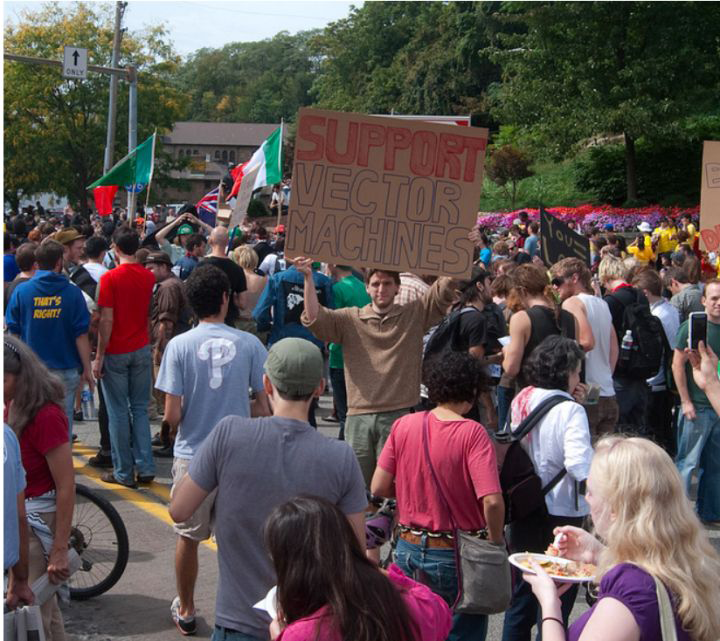
\includegraphics[width=0.5\linewidth]{partition/img/svm_0.png}  
%	\caption{this is a figure demo}
%	\label{fig:label}
	\end{figure}

\end{frame} 

\begin{frame} 
\frametitle{支持向量机}  
\begin{columns}

\column{.5\textwidth}
	\begin{itemize}
		\item SVM, 俗称支持向量机,为一种supervised learning算法,属于classification的范畴。
		\item 在数据挖掘的应用中,与unsupervised的Clustering相对应和区别。
		\item 广泛应用于机器学习(Machine Learning), 计算机视觉(Computer Vision) 和数据挖掘(Data Mining)当中。	
	\end{itemize}

\column{.5\textwidth}
	\begin{figure}[ht]
	\centering
	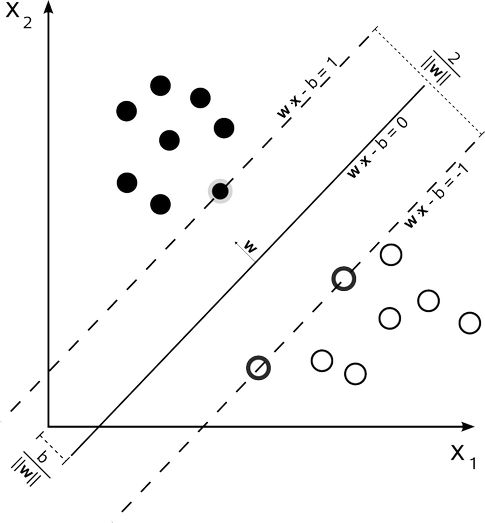
\includegraphics[width=\linewidth]{partition/img/svm_1.jpg}  
%	\caption{this is a figure demo}
%	\label{fig:label}
	\end{figure}


\end{columns}
\end{frame} 

\begin{frame}
\frametitle{一个游戏}	
现在桌子上有两种颜色的球,现在要把他们分开。
           
	\begin{figure}[ht]
	\centering
	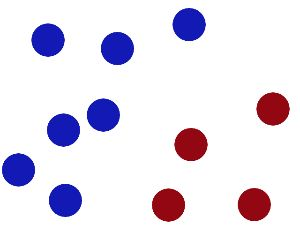
\includegraphics[width=0.5\linewidth]{partition/img/svm_2.jpg}  
%	\caption{this is a figure demo}
%	\label{fig:label}
	\end{figure}

\end{frame} 

\begin{frame}
\frametitle{一个游戏}	
我们把一根棍子放在中间,看上去干得不错。
           
	\begin{figure}[ht]
	\centering
	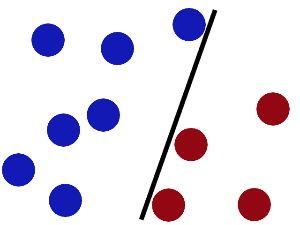
\includegraphics[width=0.5\linewidth]{partition/img/svm_3.jpg}  
%	\caption{this is a figure demo}
%	\label{fig:label}
	\end{figure}

\end{frame} 

\begin{frame}
\frametitle{一个游戏}	
有些人又往桌子上放了一些球,大部分都分对了,但是出现了一个错分的。
           
	\begin{figure}[ht]
	\centering
	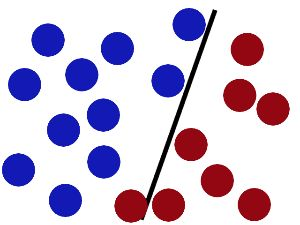
\includegraphics[width=0.5\linewidth]{partition/img/svm_4.jpg}  
%	\caption{this is a figure demo}
%	\label{fig:label}
	\end{figure}

\end{frame} 

\begin{frame}
\frametitle{一个游戏}	
SVM就是试图把棍放在最佳位置,好让在棍的两边有尽可能大的间隙。
           
	\begin{figure}[ht]
	\centering
	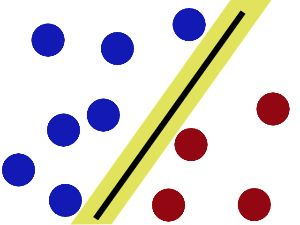
\includegraphics[width=0.5\linewidth]{partition/img/svm_5.jpg}  
%	\caption{this is a figure demo}
%	\label{fig:label}
	\end{figure}

\end{frame} 

\begin{frame}
\frametitle{一个游戏}	
现在即使放了更多的球,棍仍然是一个好的分界线
           
	\begin{figure}[ht]
	\centering
	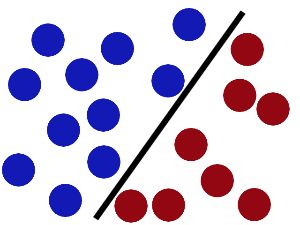
\includegraphics[width=0.5\linewidth]{partition/img/svm_6.jpg}  
%	\caption{this is a figure demo}
%	\label{fig:label}
	\end{figure}

\end{frame} 

\begin{frame}
\frametitle{一个游戏}	
 我们已经学会了一个trick,然后,在SVM 工具箱中有另一个更加重要的 trick,于是又有一个新的挑战。
           
	\begin{figure}[ht]
	\centering
	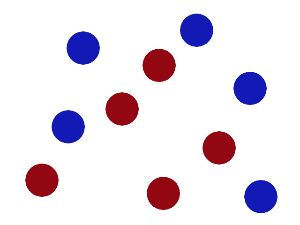
\includegraphics[width=0.5\linewidth]{partition/img/svm_7.jpg}  
%	\caption{this is a figure demo}
%	\label{fig:label}
	\end{figure}

\end{frame} 

\begin{frame}
\frametitle{一个游戏}	
现在,没有棍可以很好地分开两种球了,现在怎么办呢?我们可以一拍桌子,球飞到空中。然后,抓起一张纸,插到了两种球的中间。
           
	\begin{figure}[ht]
	\centering
	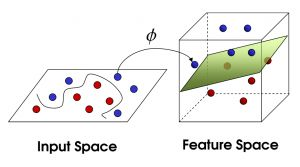
\includegraphics[width=0.5\linewidth]{partition/img/svm_8.jpg}  
%	\caption{this is a figure demo}
%	\label{fig:label}
	\end{figure}

\end{frame} 

\begin{frame}
\frametitle{一个游戏}	
现在,这些球看起来像是被一条曲线分开了。
           
	\begin{figure}[ht]
	\centering
	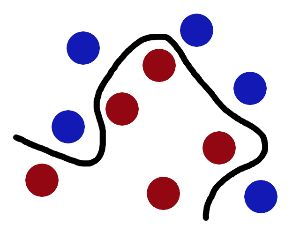
\includegraphics[width=0.5\linewidth]{partition/img/svm_9.jpg}  
%	\caption{this is a figure demo}
%	\label{fig:label}
	\end{figure}

\end{frame} 